\documentclass[12pt,twoside]{article}
\usepackage{jmlda}
\usepackage{cancel}
\newcommand{\x}{\mathbf{x}}
\newcommand{\w}{\mathbf{w}}
\newcommand{\W}{\mathbf{W}}
\newcommand{\y}{\mathbf{y}}
\newcommand{\X}{\mathbf{X}}
\newcommand{\Y}{\mathbf{Y}}
\newcommand{\fx}{\mathbf{f}}
\newcommand{\fs}{\mbox{f}}
%\NOREVIEWERNOTES
\title
    [Предсказание биологической активности ядерных рецепторов] % Краткое название; не нужно, если полное название влезает в~колонтитул
    {Вероятностный подход для задачи предсказания биологической активности ядерных рецепторов}
\author
    [Володин~С.\,Е.] % список авторов для колонтитула; не нужен, если основной список влезает в колонтитул
    {Володин~С.\,Е., Попова~М., Стрижов~В.\,В.} % основной список авторов, выводимый в оглавление
    [Володин~С.\,Е., Попова~М., Стрижов~В.\,В.] % список авторов, выводимый в заголовок; не нужен, если он не отличается от основного
\thanks
    {Работа выполнена при финансовой поддержке РФФИ, проект \No\,00-00-00000.
   Научный руководитель:  Стрижов~В.\,В.
   Задачу поставил:  Эксперт~И.\,О.
    Консультант:  Попова~М.}
\email
    {sergei.volodin@phystech.edu}
\organization
	    {Московский физико-технический институт}
\abstract
    {Решается задача предсказания биологической активности молекул протеинов (лиганд) с рецепторами: по признакам лиганда необходимо оценить вероятность связывания этой молекулы с одним или несколькими клеточными рецепторами и построить бинарный классификатор. Экспертные знания в области биохимии и фармакологии дают основания предполагать, что факты связывания одних и тех же молекул с различными рецепторами не независимы. В данной работе предлагается модель, позволяющая строить предсказания сразу для группы рецепторов, учитывая их схожесть. В работе проводится вычислительный эксперимент на реальных данных, в ходе которого предложенная модель сравнивается с независимыми моделями в терминах нескольких функционалов качества.

\bigskip
\textbf{Ключевые слова}: \emph {классификация, вероятность, classifier chains, multi-label, логистическая регрессия}.}

% TODO
% * Аннотация: какая модель предлагается и каковы ее свойства (3 предложения)
% * использовать множественный \cite{a b c}
% * Введение, 3й абзац. "решается" вместо "решена"
% * Гущин http://www.machinelearning.ru/wiki/images/5/56/Guschin2015Stacking.pdf посмотреть ссылки
% * Mixture of experts, бустинг
% * "экспоненциальное распределение" -- убрать, сделать более конкретно
% * сделать f: WxXxY выключной
% "апостериорная вероятность" -- какая?
% Постановка задачи: почему 5-fold?
% Графики Binary Relevance на одну страницу, размер каждого 0.3

\begin{document}
\maketitle
%\linenumbers
\section{Введение}
Проблема предсказания биологической активности лигандов и рецепторов является актуальной задачей в области биохимии и фармакологии \cite{hornak}, \cite{Myint2012}, \cite{Myint2015}, \cite{vinay2008}, \cite{Zhengjun5ht1a}, \cite{laurent2008}. Данная статья посвящена решению этой задачи методами машинного обучения.

Компьютерное моделирование взаимодействия молекул является распространенным методом предсказания биологической активности клеточных рецепторов \cite{vinay2008}, \cite{hornak}. Однако такой способ требует знания точной структуры лиганд, которая не всегда известна. По этой причине развитие методов машинного обучения \cite{peter1998}, позволяющих делать предсказания на основании только числовых признаков лиганд, является актуальным.

Существует два основных подхода к решению описанной задачи. В рамках первого из них для каждого клеточного рецептора строятся независимые модели. Так, например в \cite{svm}, \cite{Zhengjun5ht1a} применяется метод опорных векторов, в \cite{Myint2012} и \cite{Myint2015}~--- нейронные сети, а в \cite{scott2006}~--- метод k ближайших соседей. Второй подход подразумевает построение одной модели для предсказания активности группы рецепторов. Такой подход позволяет строить более сложные модели, учитывающие информацию о схожести рецепторов \cite{laurent2008}. В \cite{popova1} проведен сравнительный анализ обоих подходов.

Таким образом, данная задача решена многими способами. Тем не менее, как показывает сопоставление результатов \cite{popova1}, лучшим оказывается второй подход, т.е. классификаторы, учитывающие при обучении все рецепторы сразу, а не независимо друг от друга. В данном случае это означает использование нескольких классификаторов и объеднение их в <<цепочку>> \cite{elena}, \cite{weiweicc}, \cite{jesse}. Как показывает практика, обучение нескольким задачам сразу дает существенный прирост в качестве конечного алгоритма по сравнению с рассмотрением этих задач по-отдельности \cite{weiwei2010}, \cite{maxime2015}, \cite{jesse}.

В данной работе предлагается усовершенствованный метод classifier chains \cite{jesse}~--- вероятностная модель последовательного вывода для предсказания биологической активности рецепторов \cite{enrique}, \cite{weiwei2010}. Предложенный алгоритм относится ко второму подходу, то есть позволяет строить предсказания для группы рецепторов, а также допускает добавление новых без необходимости повторного обучения. Проведен вычислительный эксперимент на реальных данных, в котором набор независимых моделей сравнивался с моделью последовательного вывода. Построенные модели сравнивались по нескольким критериям качества.
\section{Постановка задачи классификации}
Задана выборка $\mathfrak{D}=\{(\x_i,\y_i)\}_{i\in \mathcal{L}}, \mathcal{L}=\{1,\dots, m\}$~--- $m$ пар объект-ответ. Каждый из объектов $\x_i\in \mathbb{R}^n$~--- вектор действительных чисел. Объект может принадлежать каждому из $l$, что представляется вектором ответов $\y_i\in \{0,1,\Box\}^l$, $1$ означает принадлежность классу, а $\Box$ означает пропуск в данных. Выборка разбита на обучающую и контрольную: $\mathfrak{D}=\mathfrak{L}\sqcup\mathfrak{T}$

%$\X=\mathbb{R}^n$~--- пространство независимых переменных (объектов), $\Y=\{0,1\}^l$~--- пространство всех ответов.

Определяются $\X, \Y$~--- случайные величины.
% на пространстве $\X\times\Y$
Считается, что между классами есть зависимости:
$$P(\Y|\X)\neq \prod_{j=1}^l P(y_j|\X)$$
Вводится предположение, что условное распределение $P(\X|\Y)$ принадлежит семейству экспоненциальных распределений.

%Рассмотрим \cite{weiwei2010} величину $P(\y|\x)=P(y_1|\x)\cdot\prod_{i=2}^lP(y_i|y_1,...,y_{i-1},\x)$~--- по свойству вероятности. Из этой формулы следует, что вероятность $P(\y|\x)$ можно найти как произведение вероятностей, причем $i$-я обусловлена по значению $i-1,...,1$ признаков.

%Моделью классификации назовем функцию $\fx\colon \W\times\X\to [0,1]^M$ вида $\fx(\w,\x)=\fx_l(\fx_{l-1}(...\fx_1(\w_1,\x_1)...))$, где $\w=(\w_1,...,\w_l)$~--- вектор параметров модели, $\W=\W_1\times\dots\times\W_l$~--- множество параметров. $\fx_1\colon\X\to\X\times[0,1]$, ..., $\fx_k\colon \X\times [0,1]^{k-1}\to\X\times [0,1]^k$. Компоненты $\fx$~--- апостериорные вероятности принадлежности объекта к соответствующему классу:

Моделью классификации называется функция $\fs\colon \W\times\X\times\Y\to [0,1]$, где $\W$~--- множество параметров, $\w\in\W$~--- вектор параметров модели. Значение $\fs$~--- апостериорая вероятность:
$$\fs(\w,\x,\y)=P(\Y=\y|\X=\x;\w)$$

%Из сделанных предположений относительно параметров распределения следует, что $P(y_j=1|x)$

Функция потерь для значения параметра $\w$ и подвыборки $\mathcal{Z}$ определяется через функцию правдоподобия модельного распределения:
$$Q(\fs|\w, \mathcal{Z})=-\sum_{(\x,\y)\in\mathcal{Z}}\log \fs(\w,\x,\y)P(\X=\x)$$

%

Требуется найти вектор параметров $\w^*\in\W$, минимизирующий $Q$ на обучающей выборке $\mathfrak{L}$:
	$$\w^*=\argmin_{\w\in\W}Q(\fs|\w,\mathfrak{L})$$

Поскольку выборка содержит пропуски, разбиения должны быть построены таким образом, чтобы в каждой подвыборке было достаточное количество объектов с известным значением каждого признака.

В качестве дополнительного критерия качества модели используются значения функционала AUC для каждого класса $j$ на контрольной выборке $\mathfrak{T}$ при 5 различных разбиениях. %:
%$$\mbox{AUC}_j(f_j,\w_j,\mathfrak{T})=\frac{1}{g_j(|\mathfrak{T}|-g_j)}\sum_{(\x,\y)\in\mathfrak{L}}\sum_{(\hat{\x},\hat{\y})\in\mathfrak{L}}[y_j<\hat{y}_j][f_j(\w_j,\x)<f_j(\w_j,\hat{\x})],$$
%где $g_j$~--- количество объектов в $\mathfrak{T}$ с $y_j=1$.

\section{Описание алгоритма}
Решим поставленную задачу, используя метод, описанный в \cite{weiwei2010}.

Докажем равенство $P(\y|\x)=\prod_{i=1}^lP(y_i|y_1,...,y_{i-1}, \x)$. Рассмотрим величину $P(y_i|y_1,...,y_{i-1},\x)=\frac{P(y_1,...,y_i,\x)}{P(y_1,...,y_{i-1},\x)}$. Подставим их в произведение, получим: $P(\y|\x)=\frac{\cancel{P(y_1,\x)}}{P(\x)}\frac{\cancel{P(y_1,y_2,\x)}}{\cancel{P(y_1,\x)}}\cdot...\cdot\frac{P(y_1,...,y_l,\x)}{\cancel{P(y_1,...,y_{l-1},\x)}}=P(\y|\x) \blacksquare$

Таким образом, для моделирования вероятности $P(\y|\x)$ можно использовать условные вероятности $P(y_1|\x),\,P(y_2|y_1,\x)...,\,P(y_l|y_1,...,y_{l-1},\x)$

Покажем, как получить из вероятности $P(\y|\x)$ вероятности классов, а также как построить бинарный классификатор, основываясь на различных функциях потерь (см. \cite{weiwei2010}).

\begin{enumerate}
\item Hamming Loss. Получаем $h_i(\x)=\sign(P(y_i=1|\x)-P(y_i=0|\x))$
\item Subset 0/1 Loss. Получаем $\y=\argmax_{y\in Y}P(\y|\x)$
\item Rank Loss. Получаем $f_i(\x)=P(y_i=1|\x)$
\end{enumerate}

Описать, как решается проблема с пропусками (классификация уже имеющимися звеньями)

Описать алгоритм обучения и классификации

Описать, как получить $P(y_i=1|\x)$ из известного $P(\y|\x)$.

Описать, как производить разбиение

Описать, как выбирать порог логистической регрессии $\frac{\lambda_+}{\lambda_-}$ по точке на ROC-кривой.

Описать, как обрабатывать пропуски (и придумать нормальный алгоритм)

\section{Вычислительный эксперимент}

%\section{Базовый вычислительный эксперимент}
Целью эксперимента является получение характеристик простого алгоритма для дальнейшего сравнения его с предлагаемым в статье. Базовый алгоритм использует подход Binary Relevance \cite{weiwei2010}, в котором зависимости между классами не учитываются. Таким образом, алгоритм представляет собой $l$ независимых логистических регрессий, по одному классификатору для каждого класса.

Эксперимент проведен на реальных данных, имеющих двойное происхождение. Объектами являются лиганды, их признаки $\x_i$ смоделированы при помощи специальной программы. Ответы $\y_i=(y_{i1},...,y_{il})$ являются результатами биохимических экспериментов, показывающих, связывается ли данный лиганд с рецептором $j$. Пропуск в ответах означает, что эксперимент либо не был проведен, либо не позволяет с достаточной уверенностью говорить о каком-либо результате. Каждый объект имеет $165$ признаков. Признаки являются химическими параметрами молекулы. В выборке содержится $8513$ объектов, количество объектов с измеренным ответом $j$ составляет около половины. В таблице \ref{t:dataDescr} указано точное распределение ответов по классам.

\begin{table}[t]%\small
	\caption{Количество связывающихся с рецепторами лигандов}
	\label{t:dataDescr}
	\centering\medskip%\tabcolsep=2pt%\small
	\begin{tabular}{lrrr}
		\headline
		
		Рецептор
		
		& Неизвестно
		& Не связывается
		& Связывается\\
		
		\headline
{\tt NR-AhR}
& $\mathbf{3413}\, (40 \%)$
& $\mathbf{4503}\, (52 \%)$
& $\mathbf{597}\, (7 \%)$\\

{\tt NR-AR-LBD}
& $\mathbf{3213}\, (37 \%)$
& $\mathbf{5129}\, (60 \%)$
& $\mathbf{171}\, (2 \%)$\\

{\tt NR-AR}
& $\mathbf{2904}\, (34 \%)$
& $\mathbf{5398}\, (63 \%)$
& $\mathbf{211}\, (2 \%)$\\

{\tt SR-MMP}
& $\mathbf{3925}\, (46 \%)$
& $\mathbf{3870}\, (45 \%)$
& $\mathbf{718}\, (8 \%)$\\

{\tt NR-ER}
& $\mathbf{3746}\, (44 \%)$
& $\mathbf{4232}\, (49 \%)$
& $\mathbf{535}\, (6 \%)$\\

{\tt SR-HSE}
& $\mathbf{3309}\, (38 \%)$
& $\mathbf{4961}\, (58 \%)$
& $\mathbf{243}\, (2 \%)$\\

{\tt SR-p53}
& $\mathbf{3174}\, (37 \%)$
& $\mathbf{5029}\, (59 \%)$
& $\mathbf{310}\, (3 \%)$\\

{\tt NR-PPAR-gamma}
& $\mathbf{3393}\, (39 \%)$
& $\mathbf{4987}\, (58 \%)$
& $\mathbf{133}\, (1 \%)$\\

{\tt SR-ARE}
& $\mathbf{3791}\, (44 \%)$
& $\mathbf{4029}\, (47 \%)$
& $\mathbf{693}\, (8 \%)$\\

{\tt NR-Aromatase}
& $\mathbf{4544}\, (53 \%)$
& $\mathbf{3835}\, (45 \%)$
& $\mathbf{134}\, (1 \%)$\\

{\tt SR-ATAD5}
& $\mathbf{2951}\, (34 \%)$
& $\mathbf{5360}\, (62 \%)$
& $\mathbf{202}\, (2 \%)$\\

{\tt NR-ER-LBD}
& $\mathbf{3107}\, (36 \%)$
& $\mathbf{5168}\, (60 \%)$
& $\mathbf{238}\, (2 \%)$\\
		\hline
	\end{tabular}
\end{table}

Для определения эффективности данного метода вычисляются значения функционала AUC для каждого из разбиений $\mathfrak{D}=\mathfrak{L}\sqcup\mathfrak{T}$ на тестовую и контрольную выборку. Разбиения выполнены по методу k-fold, где $k=5$. Вычисляется среднее значение AUC, а также стандартное отклонение.

На графиках (\ref{fg:BR1}, \ref{fg:BR2}) показаны ROC-кривые классов для одного из разбиений, а также значение функционала AUC.

%['NR-AhR' 'NR-AR-LBD' 'NR-AR' 'SR-MMP' 'NR-ER' 'SR-HSE' 'SR-p53' 'NR-PPAR-gamma' 'SR-ARE' 'NR-Aromatase' 'SR-ATAD5' 'NR-ER-LBD']

\begin{figure}[h]
	\subfloat[Рецептор NR-AhR]{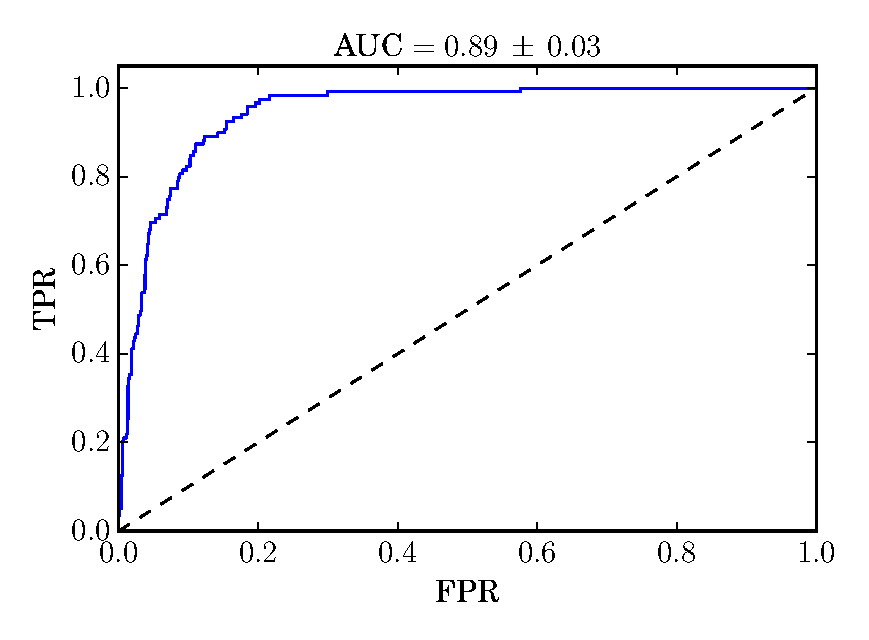
\includegraphics[width=0.5\textwidth]{class1}}
	\subfloat[Рецептор NR-AR-LBD]{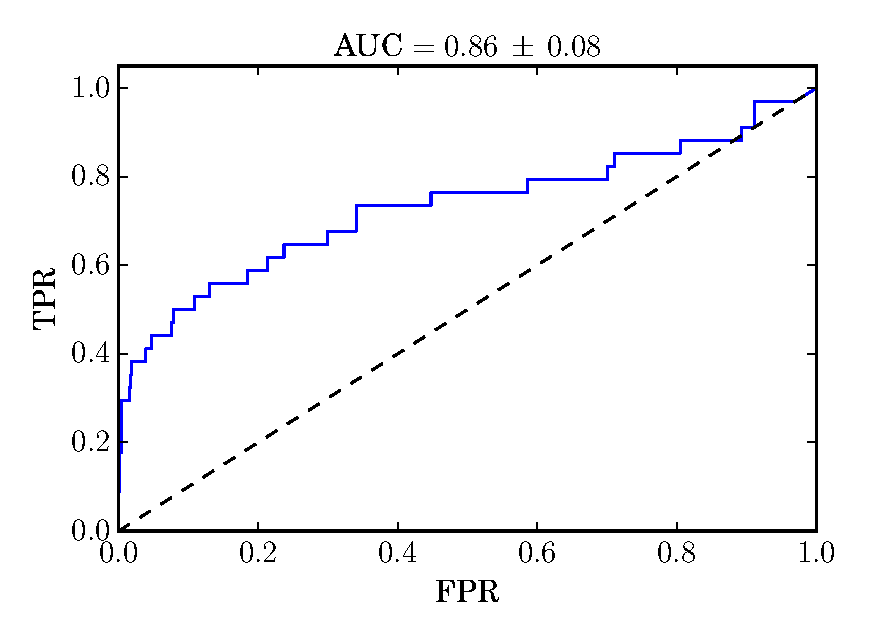
\includegraphics[width=0.5\textwidth]{class2}}\\
	\subfloat[Рецептор NR-AR]{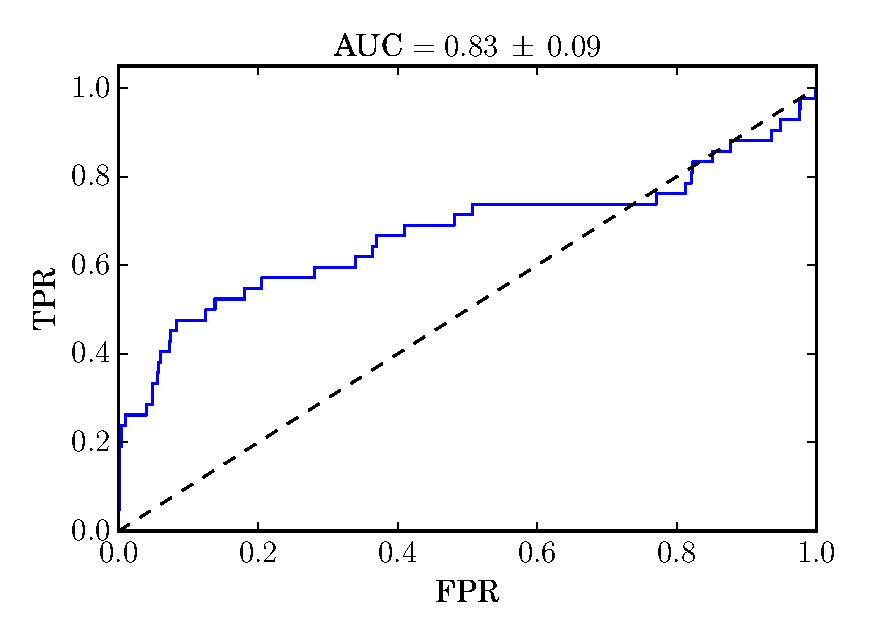
\includegraphics[width=0.5\textwidth]{class3}}
	\subfloat[Рецептор SR-MMP]{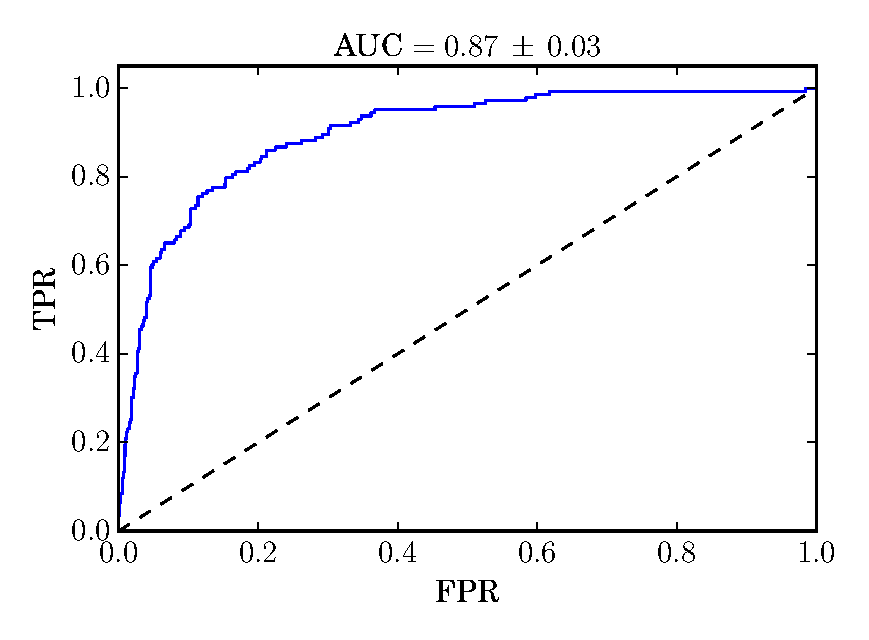
\includegraphics[width=0.5\textwidth]{class4}}\\
	\subfloat[Рецептор NR-ER]{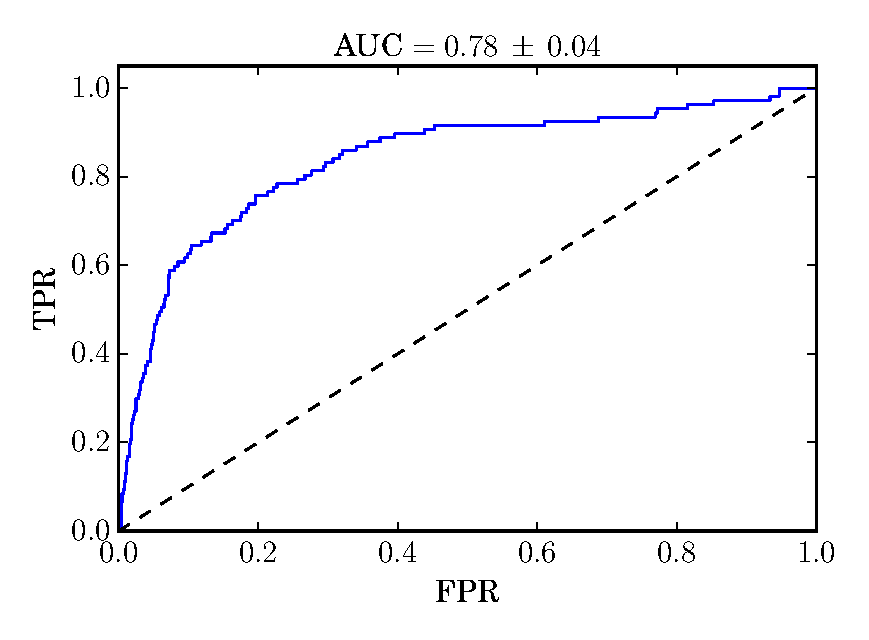
\includegraphics[width=0.5\textwidth]{class5}}
	\subfloat[Рецептор SR-HSE]{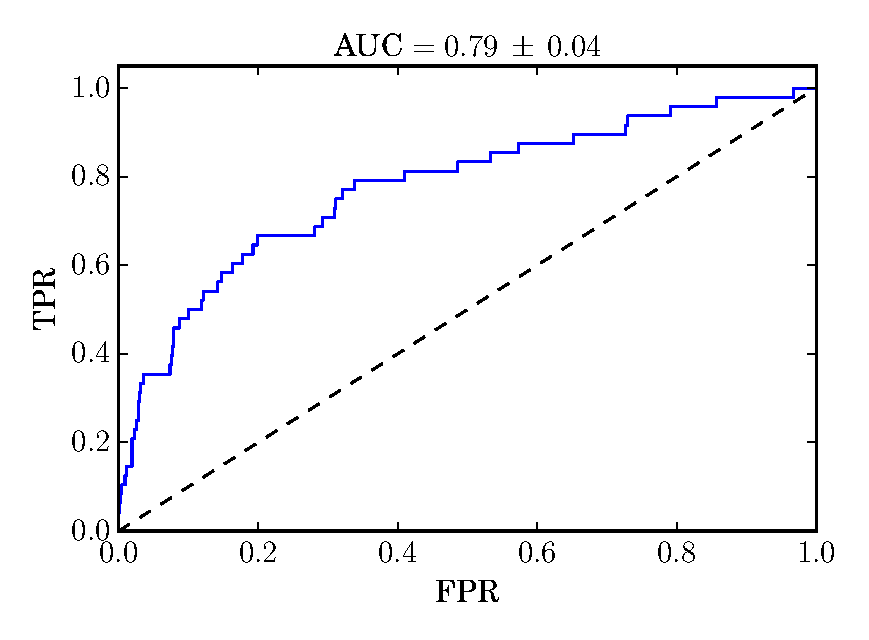
\includegraphics[width=0.5\textwidth]{class6}}\\
	\caption{ROC-кривая и значения функционала AUC для классов 1-6, метод Binary Relevance}
	\label{fg:BR1}
\end{figure}
\begin{figure}[h]
	\subfloat[Рецептор SR-p53]{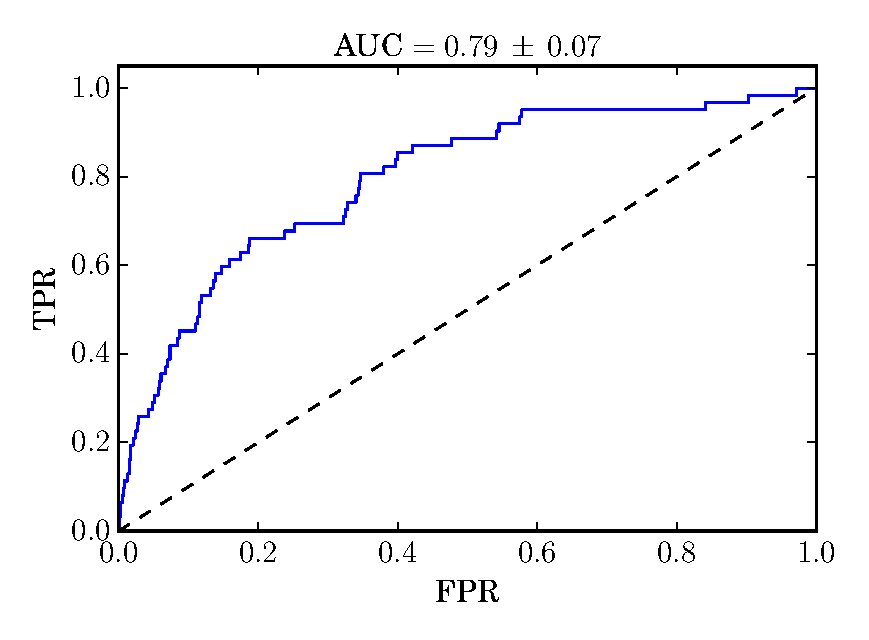
\includegraphics[width=0.5\textwidth]{class7}}
	\subfloat[Рецептор NR-PPAR-gamma]{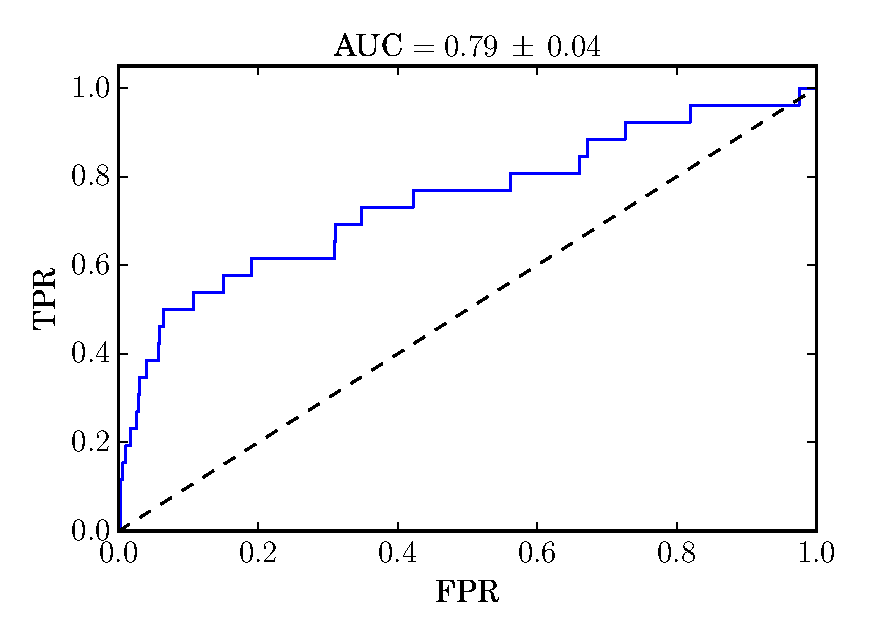
\includegraphics[width=0.5\textwidth]{class8}}\\
	\subfloat[Рецептор SR-ARE]{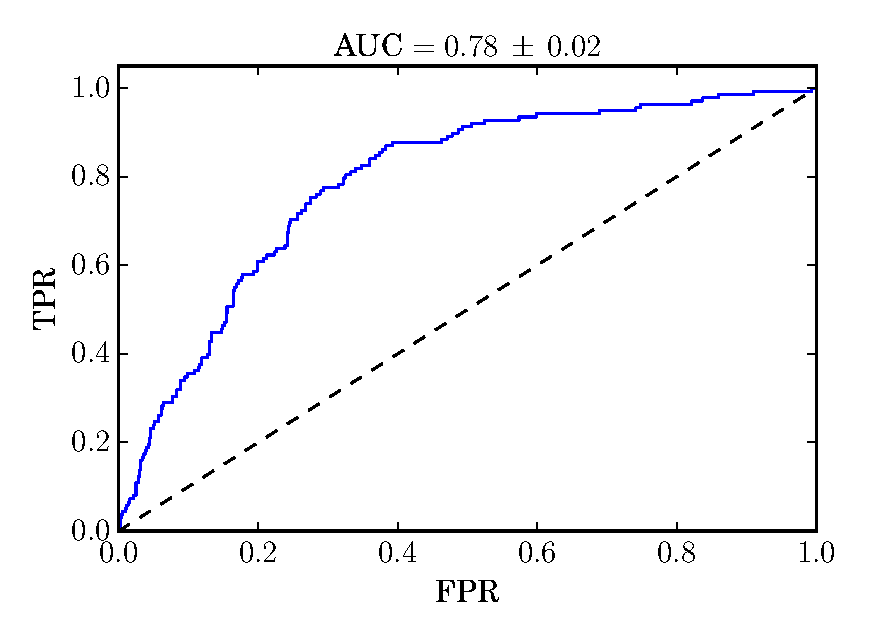
\includegraphics[width=0.5\textwidth]{class9}}
	\subfloat[Рецептор NR-Aromatase]{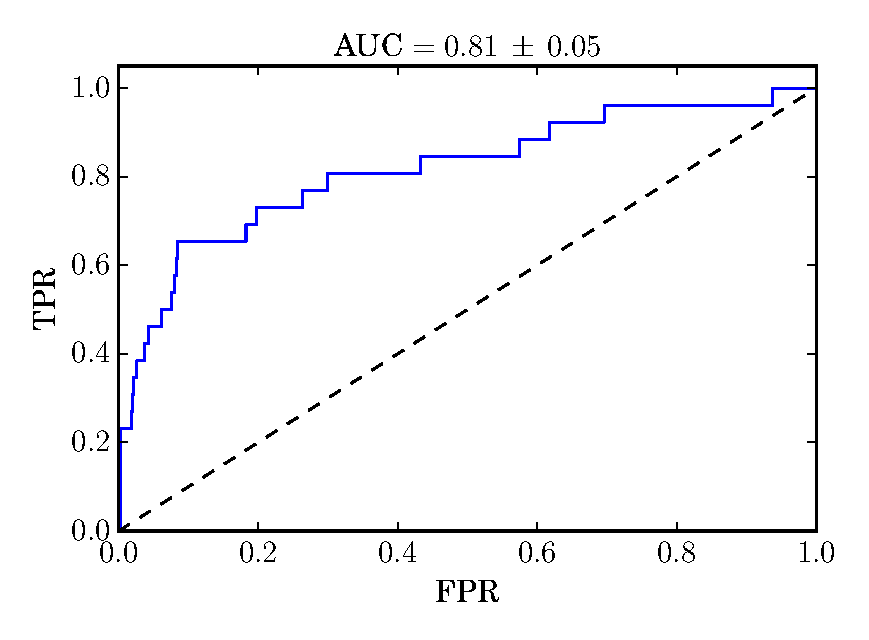
\includegraphics[width=0.5\textwidth]{class10}}\\
	\subfloat[Рецептор SR-ATAD5]{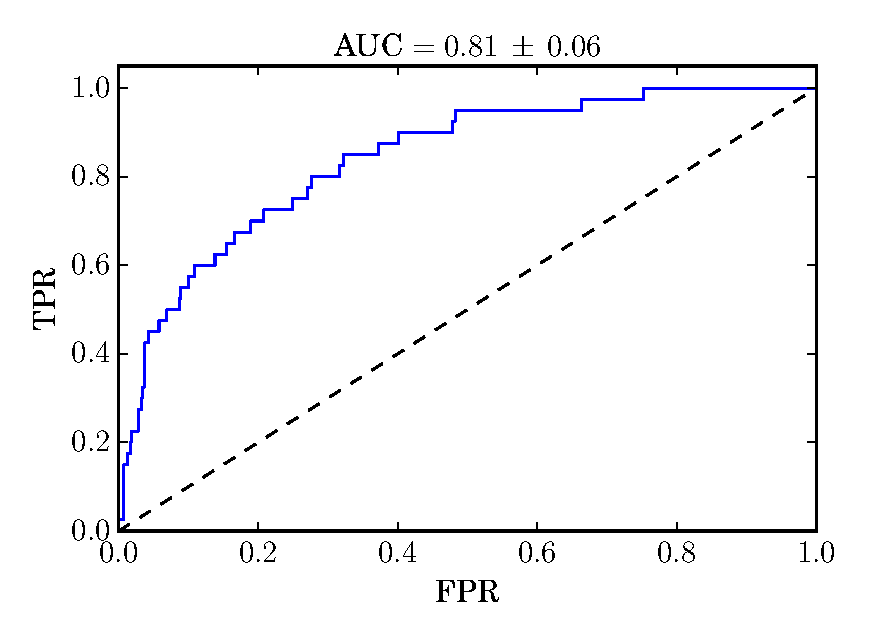
\includegraphics[width=0.5\textwidth]{class11}}
	\subfloat[Рецептор NR-ER-LBD]{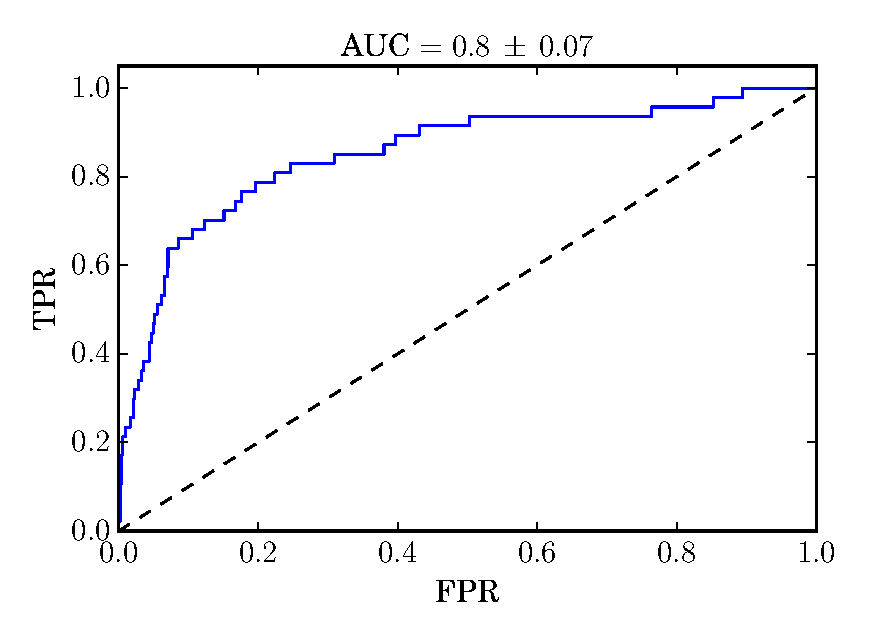
\includegraphics[width=0.5\textwidth]{class12}}
	\caption{ROC-кривая и значения функционала AUC для классов 6-12, метод Binary Relevance}
	\label{fg:BR2}
\end{figure}

В таблице \ref{t:methodCmp} приведено сравнение метода Binary Relevance с результатами из \cite{qsar}, для получения которых использовались те же данные и способ разбиения, что и в данной работе.

\begin{table}[t]%\small
\caption{Значение AUC для различных рецепторов и моделей классификации}
\label{t:methodCmp}
\centering\medskip%\tabcolsep=2pt%\small
\begin{tabular}{lrr}
\headline

Рецептор

& Binary Relevance
& Random Forest \cite{qsar} \\

\headline

{\tt NR-AhR}
& $\mathbf{0.83} \pm 0.03$
& $\mathbf{0.93}$ \\

{\tt NR-AR-LBD}
& $\mathbf{0.86} \pm 0.08$
& $\mathbf{0.88}$ \\

{\tt NR-AR}
& $\mathbf{0.83} \pm 0.09$
& $\mathbf{0.83}$ \\

{\tt SR-MMP}
& $\mathbf{0.87} \pm 0.03$
& $\mathbf{0.95}$ \\

{\tt NR-ER}
& $\mathbf{0.78} \pm 0.04$
& $\mathbf{0.81}$ \\

{\tt SR-HSE}
& $\mathbf{0.79} \pm 0.04$
& $\mathbf{0.86}$ \\

{\tt SR-p53}
& $\mathbf{0.79} \pm 0.07$
& $\mathbf{0.88}$ \\

{\tt NR-PPAR-gamma}
& $\mathbf{0.79} \pm 0.04$
& $\mathbf{0.86}$ \\

{\tt SR-ARE}
& $\mathbf{0.78} \pm 0.02$
& $\mathbf{0.84}$ \\

{\tt NR-Aromatase}
& $\mathbf{0.81} \pm 0.05$
& $\mathbf{0.84}$ \\

{\tt SR-ATAD5}
& $\mathbf{0.81} \pm 0.06$
& $\mathbf{0.83}$ \\

{\tt NR-ER-LBD}
& $\mathbf{0.80} \pm 0.07$
& $\mathbf{0.83}$ \\
\hline
\end{tabular}
\end{table}

Сравнение результатов показывает, что простой алгоритм уступает в качестве классификации методу Random Forest. Для некоторых рецепторов эта разница значительна.

\section{Заключение}

\bibliographystyle{unsrt}
\clearpage
\bibliography{Volodin2016ProbabilisticReceptorPrediction}
% Решение Программного Комитета:
%\ACCEPTNOTE
%\AMENDNOTE
%\REJECTNOTE
\end{document}
